\documentclass[12pt, twoside]{article}
\usepackage[utf8]{inputenc}
\usepackage[english,russian]{babel}
\newcommand{\hdir}{.}

\usepackage{graphicx}
\usepackage{caption}
\usepackage{amssymb}
\usepackage{mathrsfs}
\usepackage{euscript}
\usepackage{upgreek}
\usepackage{array}
\usepackage{theorem}
\usepackage{graphicx}
\usepackage{subfig}
\usepackage{caption}
\usepackage{color}
\usepackage{url}
\usepackage{amsmath}

\DeclareMathOperator*{\argmax}{arg\,max}
\DeclareMathOperator*{\argmin}{arg\,min}

\usepackage[left=2cm, right=2cm, top=3cm, bottom=3cm, bindingoffset=0cm]{geometry}

\newcommand{\Pb}{\mathcal{P}}

\setcounter{secnumdepth}{-1}

\begin{document} 

\title{Задание 2 по курсу "Байесовский выбор модели"}
\author{Грабовой Андрей, группа 574}
\date{}
\maketitle

\section{Задача 1}
Пусть $\textbf{x} \in \mathbb{R}^n:~\forall i\in\{0,...,n\}~x_i\in N(m,\sigma)$. Проверить гипотезу $H_0$  о том, что $m=0$. Вычислить критическую область и сосчитать мощность критерия $W$ от истиных $m$ и $\sigma$.\\

1. Рассмотрим следующую статистику:
$$T(\textbf{x}) = \frac{\bar{\textbf{x}}}{\frac{\bar{\sigma}}{\sqrt{n+1}}} \sim t(n)~\text{--- в условии истиност гипотезы}$$

2. Критическая область $|T(\textbf{x})| \le t_{\text{кр}}(\alpha, n)$, где $t_{\text{кр}}(\alpha, n) = |F_{t(n)}^{-1}(\frac{\alpha}{2})|$. Для $n = 100$ и $\alpha = 0.05$ показано на рис.~\ref{first}:

\begin{figure}[h!]\center
{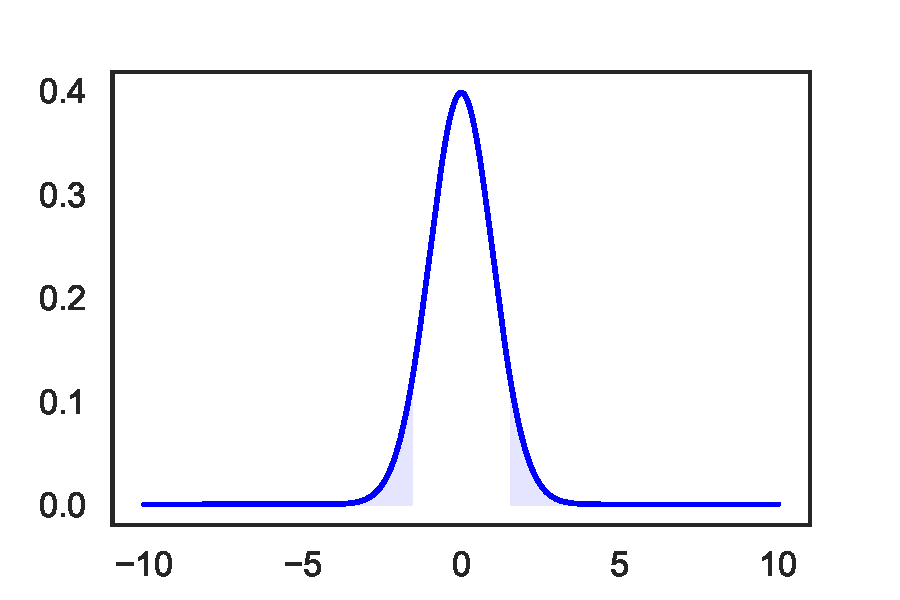
\includegraphics[width=0.8\textwidth]{first}}
\caption{График критической области}
\label{first}
\end{figure}

3. Мощность критерия это просто площадь под графиком(красная), как показано на рис.~\ref{first_pow}:
\begin{figure}[h!]\center
{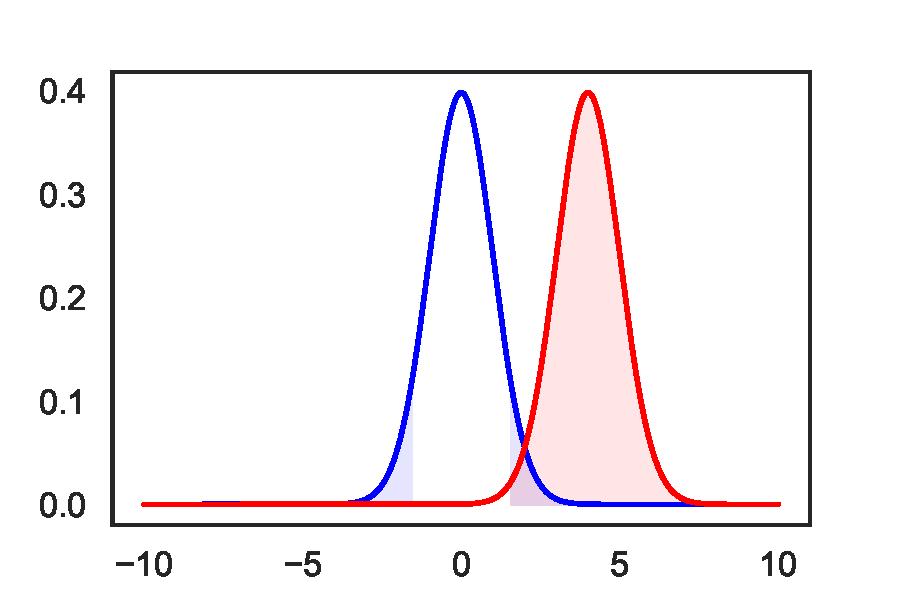
\includegraphics[width=0.8\textwidth]{first_pow}}
\caption{График критической области}
\label{first_pow}
\end{figure}

$$W = \left(\int_{-\infty}^{-t_{\text{кр}}(\alpha, n)}+\int^{\infty}_{t_{\text{кр}}(\alpha, n)}\right)p_{t(n) + \frac{m_0\sqrt{n+1}}{\bar{\sigma}}}(x)dx = $$
$$=  \left(\int_{-\infty}^{-t_{\text{кр}}(\alpha, n)}-\int_{-\infty}^{t_{\text{кр}}(\alpha, n)}\right)p_{t(n) + \frac{m_0\sqrt{n+1}}{\bar{\sigma}}}(x)dx + 1 = $$
$$= 1 + F_{t(n) +\frac{m_0\sqrt{n+1}}{\bar{\sigma}}}(-{t_{\text{кр}}(\alpha, n)}) - F_{t(n) +\frac{m_0\sqrt{n+1}}{\bar{\sigma}}}({t_{\text{кр}}(\alpha, n)}) $$

\section{Задача 2}
Заметим:
$$p(\textbf{y}, \textbf{w}, \textbf{X}|\alpha) = p(\textbf{y}, \textbf{w}|\textbf{X},\alpha)p(\textbf{X})\Rightarrow p(\textbf{y}, \textbf{w}|\textbf{X},\alpha) = p(\textbf{w}|\alpha)p(\textbf{y}|\textbf{w}, \textbf{X})$$
1. 
$$p(\textbf{y}_\text{test}|\textbf{X}_\text{test}, \textbf{X}_\text{train}, \textbf{y}_\text{train}) = \int p(\textbf{y}_\text{test}, \textbf{w}|\textbf{X}_\text{test}, \textbf{X}_\text{train}, \textbf{y}_\text{train}) d\textbf{w}=$$
$$ = \int p(\textbf{y}_\text{test}|\textbf{w}, \textbf{X}_\text{test})p(\textbf{w}|\textbf{X}_\text{train}, \textbf{y}_\text{train})d\textbf{w} = \int p(\textbf{y}_\text{test}|\textbf{w}, \textbf{X}_\text{test}) \frac{p(\textbf{w})p(\textbf{X}_\text{train}, \textbf{y}_\text{train}| \textbf{w})}{p(\textbf{X}_\text{train}, \textbf{y}_\text{train})}d\textbf{w}=$$

$$= \int p(\textbf{w})p(\textbf{y}_\text{test}|\textbf{w}, \textbf{X}_\text{test})p(\textbf{y}_\text{train}|\textbf{w}, \textbf{X}_\text{train}) \frac{p(\textbf{X}_\text{train})}{p(\textbf{X}_\text{train}, \textbf{y}_\text{train})}d\textbf{w} =$$
$$= \int \frac{p(\textbf{w})p(\textbf{y}_\text{train}|\textbf{w}, \textbf{X}_\text{train}) }{\int p(\textbf{y}_\text{train}| \textbf{w}, \textbf{X}_\text{train})p(\textbf{w})d\textbf{w} }p(\textbf{y}_\text{test}|\textbf{w}, \textbf{X}_\text{test})d\textbf{w}$$

Тогда, прогнозируемые вероятности для $\textbf{y}_\text{test}$ являються:
$$\Pb(\textbf{y}_\text{test} = 1|\textbf{X}_\text{test}) = \int \frac{p(\textbf{w})p(\textbf{y}_\text{train}|\textbf{w}, \textbf{X}_\text{train}) }{\int p(\textbf{y}_\text{train}| \textbf{w}, \textbf{X}_\text{train})p(\textbf{w})d\textbf{w} }p(\textbf{y}_\text{test}|\textbf{w}, \textbf{X}_\text{test})d\textbf{w}$$
Истиные вероятности для $\textbf{y}_\text{test}$ являються:
$$\Pb(\textbf{y}_\text{test} =1) = \frac{1}{1+\text{exp}(-\textbf{w}^\text{T}\textbf{X}_\text{test})}$$
Так-как нам известно, что $\textbf{w} \sim N(0, \alpha^{-1}\textbf{I})$, то мы можем вычислить этот интеграл.
\section{Задача 3}
$\textbf{a.}$ Докажем, что Accuracy(ACC) является частным случаем ASY(\textbf{P}):\\

$$Acc = \frac{m_{11}+m_{00}}{m_2} = \frac{1}{m_2}\left(\sum_{i=1}^{m_{00}}1  + \sum_{i=1}^{m_{11}}1 + \sum_{i=1}^{m_{01}}0  + \sum_{i=1}^{m_{10}}0\right) =$$
$$= \left(\sum_{i=1}^{m_{00}}\frac{1}{m_2}  + \sum_{i=1}^{m_{11}}\frac{1}{m_2} + \sum_{i=1}^{m_{01}}0  + \sum_{i=1}^{m_{10}}0\right) = $$
$$= \left(\sum_{i=1}^{m_{00}}\frac{1}{m_2}  + \sum_{i=1}^{m_{11}}\frac{1}{m_2} + \sum_{i=1}^{m_{01}}0  + \sum_{i=1}^{m_{10}}0\right) = -\sum_{i=1}^{m_2}p_{y_i\hat{y}_i}$$
Знак минус появился в последнем равенстве из-за того, что ACC  мы максимизируем, а ASY минимизируем. Получаем, что ACC частный случай  ASY($\mathbf{P}$), когда 
$\mathbf{P}=
\begin{bmatrix} 
-\frac{1}{m2} &0\\
0&-\frac{1}{m2}\\
\end{bmatrix}$\\
$\textbf{b.}$ Пусть класс объектов $y_j$ не зависит от $\textbf{x}_j$:\\

1. Построить наилучший прогноз $\hat{\textbf{y}}_2$ в терминах ACC, если $\mathbb{P}(y_j = 1) = p$.\\
Наилучший прогноз достигается просто на константном классификаторе, причем за константу берем тот класс который имеет большую вероятность.\\

2. Построить наилучший прогноз $\hat{\textbf{y}}_2$ в терминах ASY(\textbf{P}), если $\mathbb{P}(y_j = 1) = p$.\\
Наилучший прогноз достигается просто на константном классификаторе. Пусть 
$\mathbf{P}=\begin{bmatrix} 
w_{00} & w_{01}\\
w_{10} & w_{11}\\
\end{bmatrix}$\\
Тогда нужно классифицировать константой $c = \argmin_{i}\left((1-p)w_{i0} + pw_{i1}\right)$ 

3. Так-как $y_j$ не зависит от $\textbf{x}_j$, то просто считаем частоты каждого класса и это будет наша оценка вероятности.

\section{Задача 4}
Пусть имеется выборка $\textbf{X}^0 = \textbf{x}^0_1, ..., \textbf{x}^0_{m_0}$ объектов класса 0 размера $m_0$ и выборка $\textbf{X}^1 = \textbf{x}^1_1, ..., \textbf{x}^1_{m_1}$ объектов класса 1 размера $m_1$. Пусть признаки независимы в совокупност в обеих выборках, а также признаки имеют нормальное распределение с дисперсиями $\sigma^2_j$, одинаковой для одного  итого же признака в разных классах, и возможно разной между признаками. Пусть требуется проверить гипотезу о том, что мат. ожидание значения признака с номером $j$  совпадают для обоих классов.\\
1. Пусть $\sigma_j = \sigma$. Проверить гипотезу о равенстве мат. ожиданий.\\
Будем проверять гипотезу о равенстве мат. ожиданий для каждого признака по отдельности.
$$\bar{\textbf{x}}^0_j \sim N(M^0_{j}, \frac{\sigma^2}{m_0}), \quad \bar{\textbf{x}}^1_j \sim N(M^1_{j}, \frac{\sigma^2}{m_1}),$$
где $M^0_j$ и $M^1_j$ --- мат. ожидание $j$-го признака для класса $0$ и класса $1$ соответственно. Тогда построим статистику  
$$T(\textbf{X})= \frac{\bar{\textbf{x}}^0_j - \bar{\textbf{x}}^1_j}{\sigma\sqrt{\frac{m_0+m_1}{m_0m_1}}} \sim N(0,1)~\text{--- в условиях истиности гипотезы}$$
Критическая область будет $|T(\textbf{X})| > t_{N(0,1)}(0.05) = [\text{по таблице}] = 1.960$.\\
2. Не могу придумать ничего лучше, чем следующее. Мы знаем, что дисперсия в классе $0$  и в классе $1$ равны, следовательно оценим $\sigma$ как среднее значение между выборочной дисперсией в классе $0$ и выборочной дисперсией в классе $1$, а дальше применим идеи использованы в пункте 1.\\
3. На рис.~\ref{forth_p} показан график зависимости $p_{value}$ от размера выборки. Из графика видно, что при увеличении размера выборки $p_{value}$ для  статистики где разность мат. ожиданий равно $1$ убывает, и при размере выборки $1000$  меньше чем 0.05. На рис.~\ref{forth_FP} и рис.~\ref{forth_TP} показано, как меняется количество ложных положительных отклонений и  настоящих положительных отклонений разности матожиданий от нуля. Как видно из графиков при увеличении размера выборки мы все верно отвергаем гипотезу или говорим, что данные не противоречат ей. В эксперименте были выбраны следующие $m_1$ и $m_2$ из табл.~\ref{table1}\\
4. 
\begin{figure}[h!]\center
{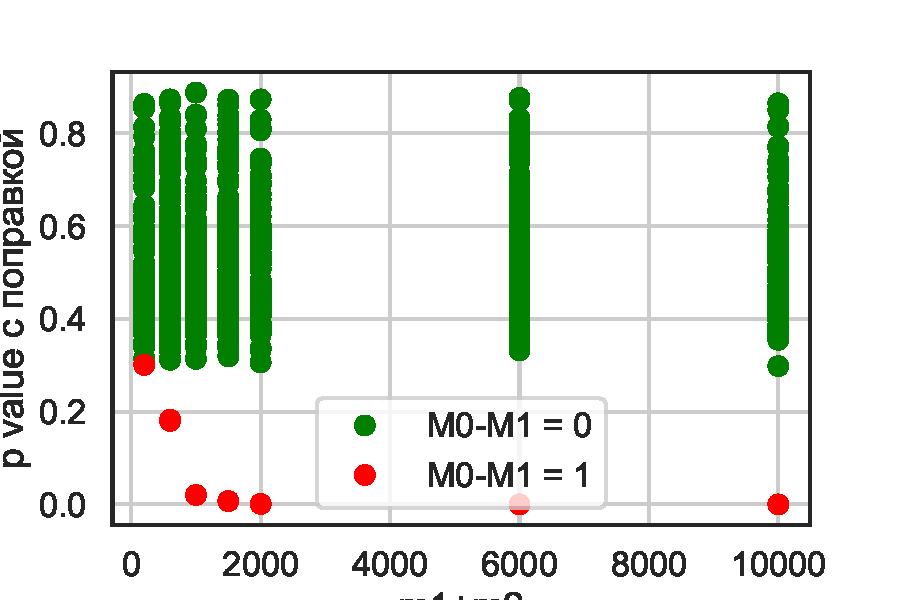
\includegraphics[width=0.8\textwidth]{forth_p}}
\caption{График зависимости $p_{value}$ от размера выборки($m_1+m_2$)}
\label{forth_p}
\end{figure}
\begin{figure}[h!]\center
{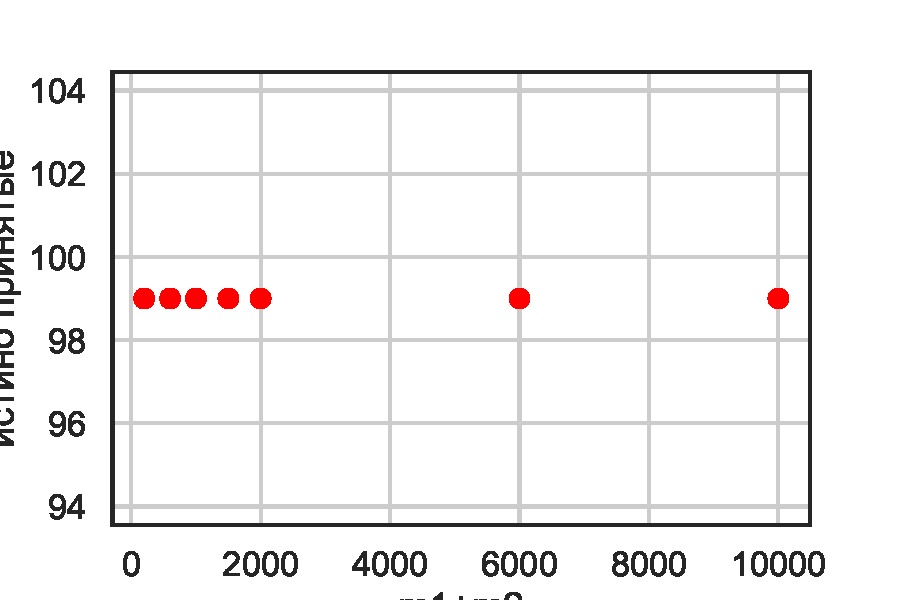
\includegraphics[width=0.8\textwidth]{forth_TP}}
\caption{График зависимости настоящих положительных отклонений от размера выборки($m_1+m_2$)}
\label{forth_TP}
\end{figure}
\begin{figure}[h!]\center
{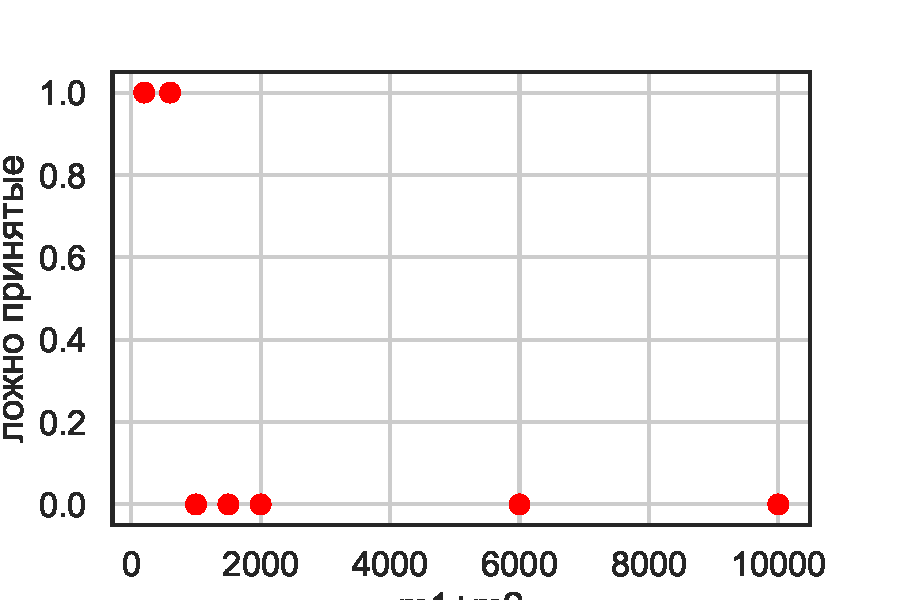
\includegraphics[width=0.8\textwidth]{forth_FP}}
\caption{График зависимости ложных положительных отклонений от размера выборки($m_1+m_2$)}
\label{forth_FP}
\end{figure}
\begin{table}[h!]
\begin{center}
\begin{tabular}{|c|c|c|c|c|c|c|c|c|c|c|}
\hline
	$m_1$ & 100 & 500 & 1000 & 5000 & 100 & 500 & 1000 & 500 & 5000 & 1000 \\
	\hline
	$m_2$ & 100 & 500 & 1000 & 5000 & 500 & 100 & 500 & 1000 & 1000 & 5000 \\
	\hline
	$m_1 + m_2$ & 200 & 1000 & 2000 & 10000 & 600 & 600 & 1500 & 1500 & 6000 & 6000 \\
\hline
\end{tabular}
\end{center}
\caption{Таблица размера выборок}
\label{table1}
\end{table}

\section{Задача 5}
1. PCA - это один из способов уменьшение размерности данных, потеряв наименьшее количество информации. По сути это просто проекция на подпространство где важные признак выбираться из svd разложения(а именно оставляем те признаки которые имеют максимальные сингулярные числа). Формально решает задачу поиска подпространства меньшей размерности, в ортогональной проекции на которые среднеквадратиченое расстояние между точками максимально. В вероятностной постановке он говорит, что нужно найти такой базис в котором матрица ковариациии диагональна\\
2. Будем предполагать, что m>>n. Тогда в силу того, что выборка независима, воспользовавшись определением, что PCA это <<Поиск ортогональных проекций с наибольшим рассеянием>>, получаем что все рассеяния одинаковые, следовательно все компоненты важны и следовательно все компоненты нужны, причем std по каждой компоненте это $\sigma$\\
3. Пусть $\textbf{X}$ состоит из n-1 зашумленной копии некоторого признака $\bf{\chi}_1$, а также из шкалированного признака $\bf{\chi}_2$, то есть  $\textbf{X} = [\bf{\chi}_1 +\varepsilon_1, \bf{\chi}_1 +\varepsilon_2, ..., \bf{\chi}_1 +\varepsilon_{n-1}, \xi \bf{\chi}_2]$, где все элементы независимым и одинаково нормально распределены. Найти в зависимости от $\xi$ ожидаемую первую главную компоненту матрицы $\textbf{X}$.\\

\begin{figure}[h!]\center
{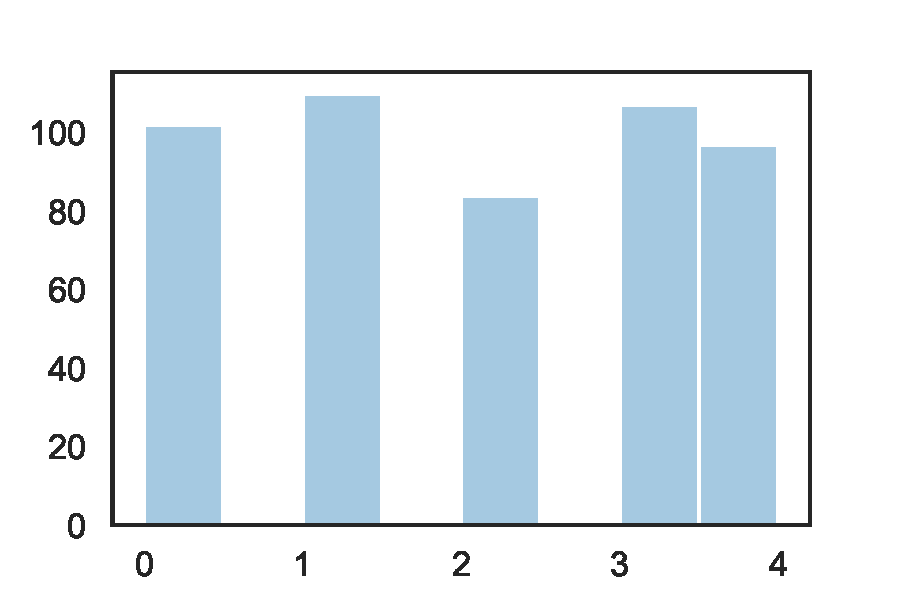
\includegraphics[width=0.8\textwidth]{fifth_1}}
\caption{Гистограмма номеров главных компонент}
\label{fifth_1}
\end{figure}

\begin{figure}[h!]\center
{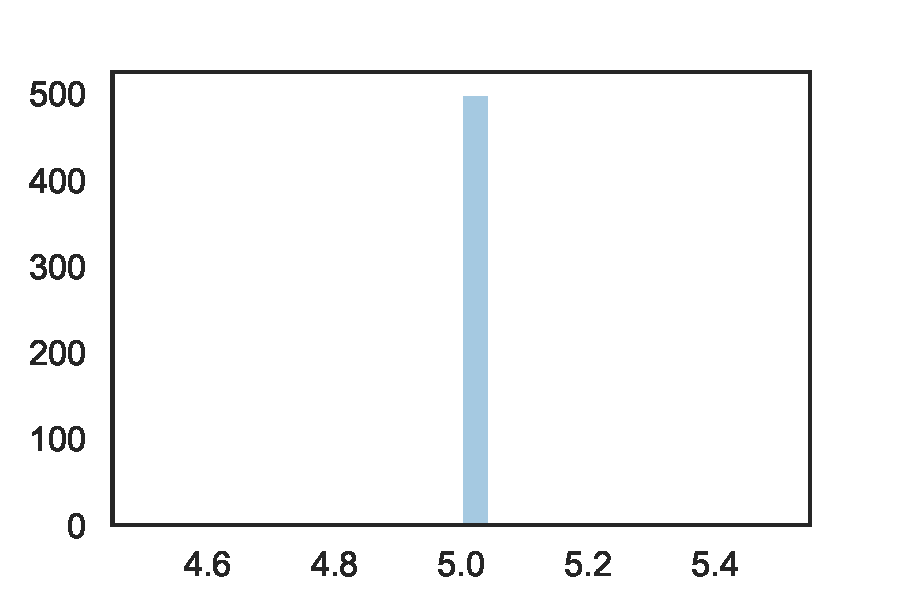
\includegraphics[width=0.8\textwidth]{fifth_3}}
\caption{Гистограмма номеров главных компонент}
\label{fifth_3}
\end{figure}

3.1. Аналитически:\\
Из определения следует, что первая главная компонента, эта компонента которая имеет максимальное среднеквадратическое отклоенние. Первые $n-1$ компоненты имеют среднеквадратические отклонения равные 2, последняя компонента имеет $\xi$. Тоесть ожидание первой главной компоненты при $\xi < 2$ это любая из $1,...n-1$, а при $\xi >= 2$ это $n$-я компонента.\\
	
3.2. Сэмплирование:\\
Рассмотрим выборку из 5 признаков порожденной по тому как описано в условии задачи. Посмотрим какая будет главная компонента для k=1 --- рис.~\ref{fifth_1} и для k=3 --- рис.~\ref{fifth_3}. Сэмплированый и аналитический результат совпадают. 


\end{document} 